\documentclass[11pt,a4paper]{article}

% Packages
\usepackage[utf8]{inputenc}
\usepackage[margin=1in]{geometry}
\usepackage{graphicx}
\usepackage{float}
\usepackage{enumitem}
\usepackage{xcolor}
\usepackage{hyperref}
\usepackage{titlesec}
\usepackage{fancyhdr}
\usepackage{tcolorbox}
\usepackage{listings}
\usepackage{booktabs}
\usepackage{array}

% Graphics path
\graphicspath{{./}}

% Color definitions
\definecolor{primarycolor}{RGB}{41, 128, 185}
\definecolor{secondarycolor}{RGB}{52, 73, 94}
\definecolor{lightgray}{RGB}{245, 245, 245}

% Hyperref setup
\hypersetup{
    colorlinks=true,
    linkcolor=primarycolor,
    filecolor=primarycolor,
    urlcolor=primarycolor,
    citecolor=primarycolor
}

% Header and footer
\pagestyle{fancy}
\fancyhf{}
\fancyhead[L]{\small\textit{Slaughter \& Butchery Module}}
\fancyhead[R]{\small\textit{System Overview}}
\fancyfoot[C]{\thepage}
\renewcommand{\headrulewidth}{0.5pt}
\renewcommand{\footrulewidth}{0.5pt}

% Title formatting
\titleformat{\section}
{\color{primarycolor}\Large\bfseries}
{\thesection}{1em}{}[\titlerule]

\titleformat{\subsection}
{\color{secondarycolor}\large\bfseries}
{\thesubsection}{1em}{}

% Document information
\title{
    \vspace{-2cm}
    {\Huge\textbf{Slaughter \& Butchery Module}}\\[0.5cm]
    {\Large System Overview}\\[1cm]
    {\large Uganda Livestock Information Tracking System (U-LITS)}
}
\author{
    \textbf{Prepared by:}\\[0.3cm]
    Mr. Muhindo Mubaraka\\
    Samuel Ocen
}
\date{December 4, 2025}

\begin{document}

\maketitle
\thispagestyle{empty}

\begin{abstract}
This document provides a comprehensive overview of the Slaughter and Butchery module within the Uganda Livestock Information Tracking System (U-LITS). The module tracks the complete livestock processing chain from farm to consumer, ensuring end-to-end traceability, quality assurance, and regulatory compliance for meat production.
\end{abstract}

\newpage
\tableofcontents
\newpage

\section{Introduction}

The Slaughter and Butchery module tracks the complete livestock processing chain from farm to consumer. It provides end-to-end traceability, quality assurance, and regulatory compliance for meat production.

\subsection{Process Overview}

The complete workflow follows this sequence:

\begin{center}
\textbf{Movement Permit $\rightarrow$ Slaughter House $\rightarrow$ Carcass Processing $\rightarrow$ Quarters $\rightarrow$ Meat Cuts $\rightarrow$ Final Products $\rightarrow$ Sale}
\end{center}

\section{Movement Permit}

\subsection{Purpose}

Movement Permits authorize and document the transport of livestock from farms to slaughter houses or between farms. This ensures proper documentation and tracking during transit.

\subsection{Process}

The movement permit process follows these steps:

\begin{enumerate}[leftmargin=*]
    \item Farmer or trader applies through mobile app or web portal
    \item Selects animals by E-ID (Electronic ID) or V-ID (Visual ID)
    \item Specifies destination (slaughter house or farm)
    \item District Veterinary Officer reviews and approves or rejects the application
    \item System generates permit with unique number and QR code
    \item Animals are transported with accompanying permit document
\end{enumerate}

\begin{figure}[h]
\centering
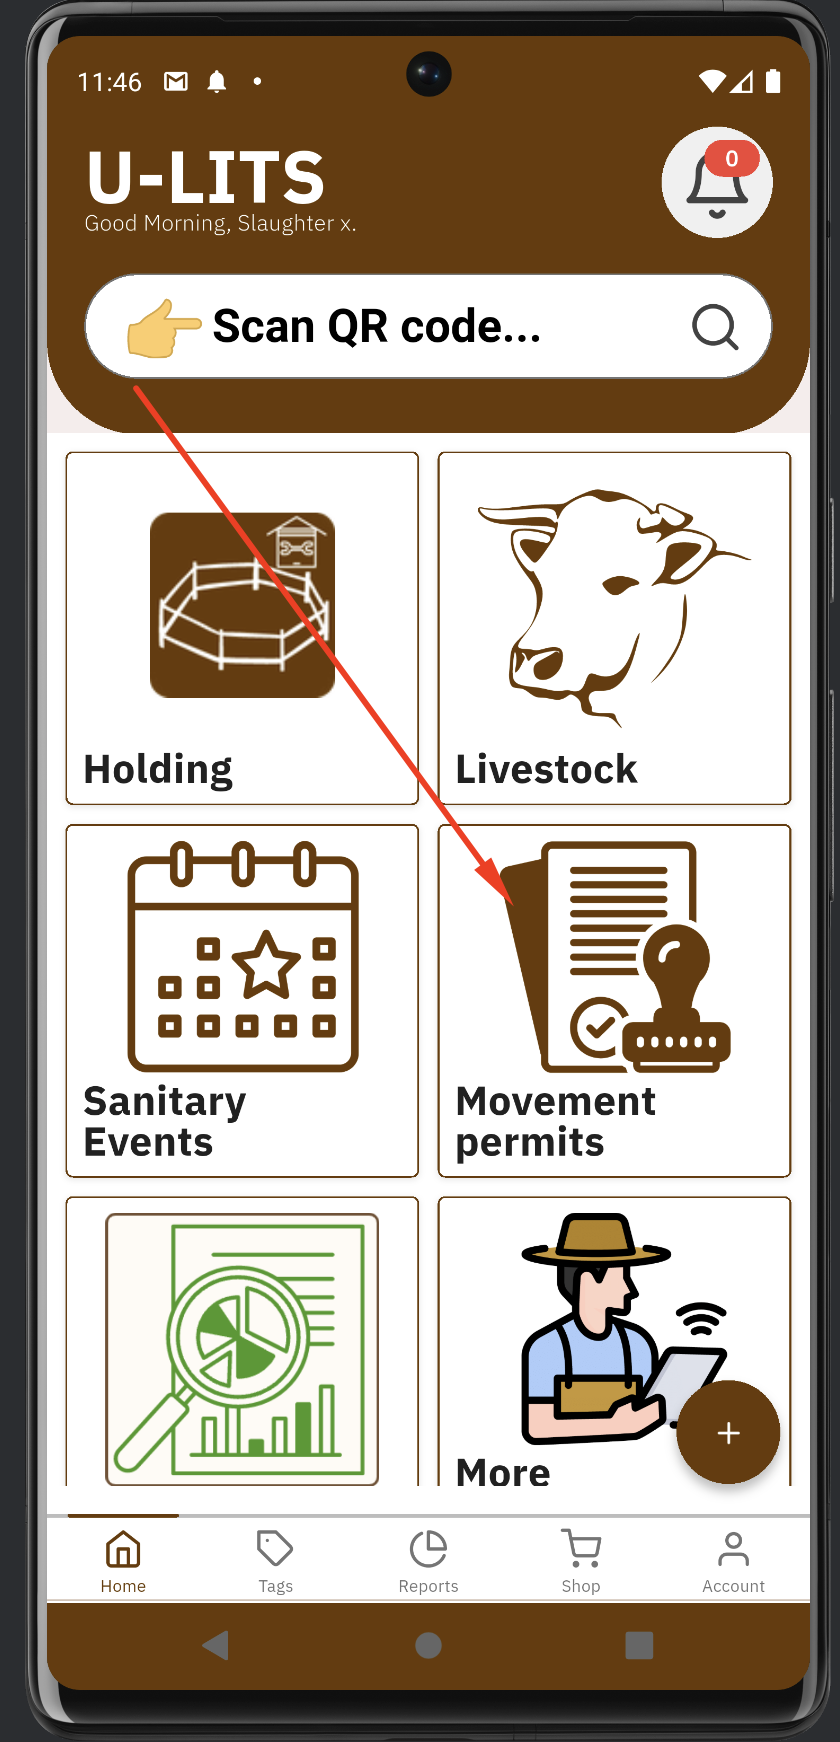
\includegraphics[width=0.45\textwidth]{01_movement_permit_application.png}
\caption{Accessing Movement Permit Module from Home Page}
\label{fig:movement_permit_app}
\end{figure}

\begin{figure}[h]
\centering
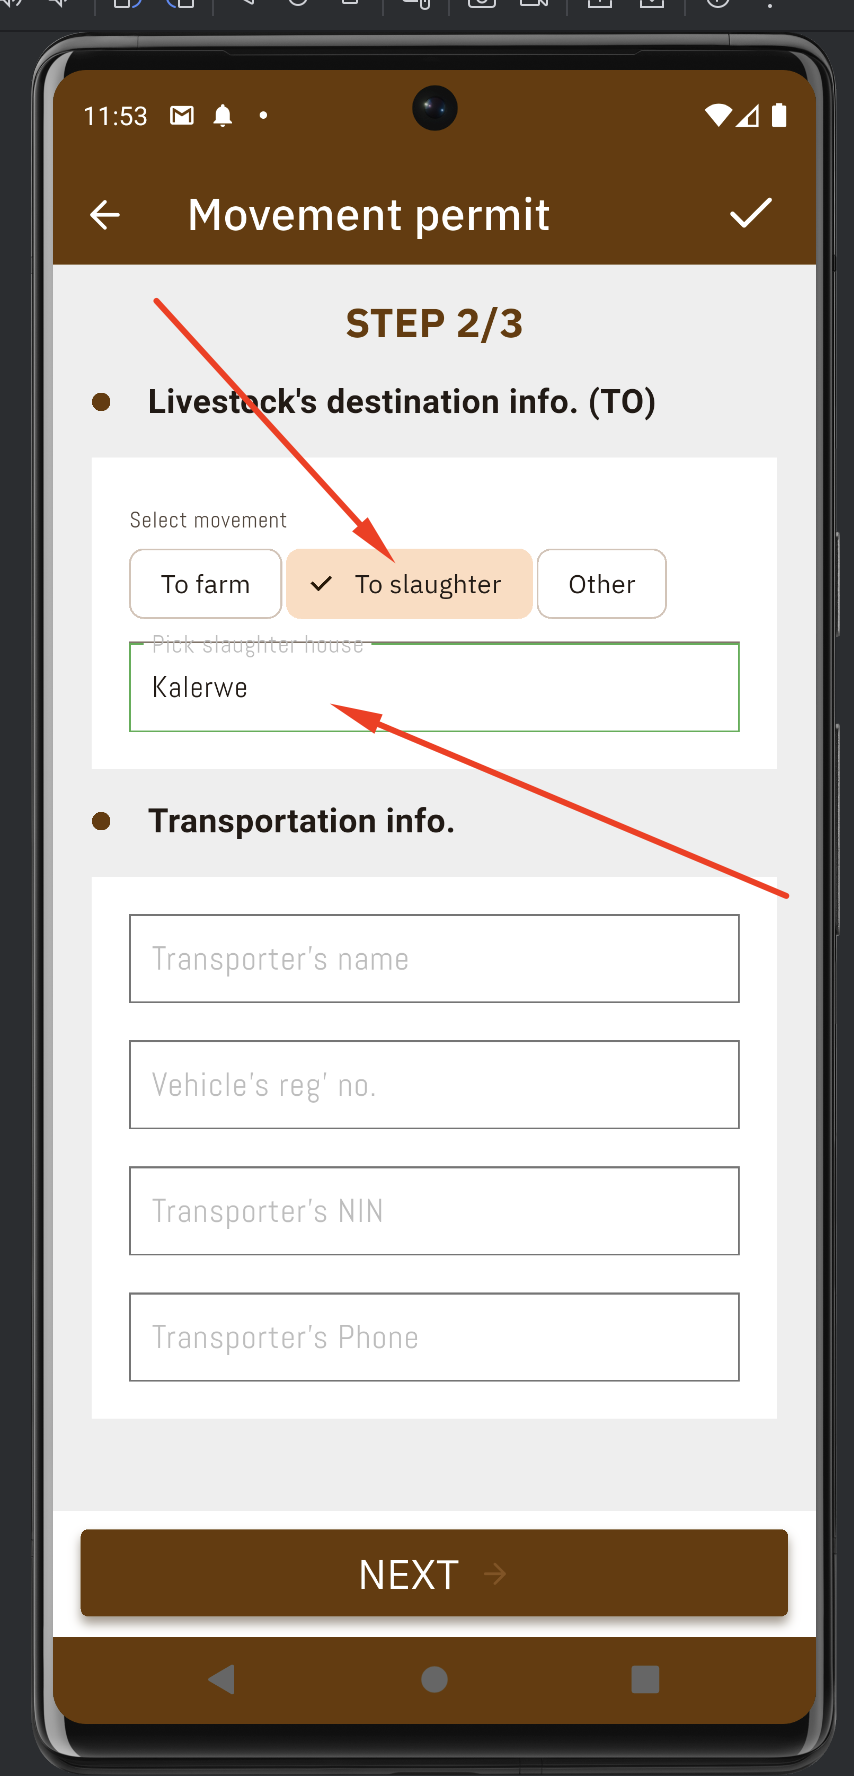
\includegraphics[width=0.45\textwidth]{02_movement_permit_form_destination.png}
\caption{Movement Permit Application Form - Selecting Destination Slaughter House}
\label{fig:movement_permit_form}
\end{figure}

\subsection{Key Information Tracked}

The system tracks the following information for each permit:

\begin{itemize}[leftmargin=*]
    \item Origin and destination locations
    \item Animal identification (E-ID, V-ID, breed, sex, age)
    \item Transport details (vehicle, route, checkpoints)
    \item Validity period
    \item Approval status
\end{itemize}

\subsection{Requirements}

\begin{itemize}[leftmargin=*]
    \item Animals must have proper identification tags
    \item Health inspections required before movement
    \item Permit approval mandatory before transport
    \item Animal list cannot be modified during transit
    \item Subject to checkpoint inspections
\end{itemize}

\section{Slaughter House Operations}

\subsection{Animal Reception}

Upon arrival at the slaughter house, staff verify:

\begin{itemize}[leftmargin=*]
    \item Movement permit is valid and approved
    \item Animals match permit details
    \item Animals are fit for slaughter
\end{itemize}

\subsection{Antemortem Inspection}

A veterinary officer examines live animals for:

\begin{itemize}[leftmargin=*]
    \item Overall health condition
    \item Disease signs or injuries
    \item Fitness for slaughter
    \item Unfit animals are rejected
\end{itemize}

\subsection{Slaughter Process}

The slaughter process includes:

\begin{itemize}[leftmargin=*]
    \item Only approved animals proceed
    \item Barcode generated for carcass tracking
    \item Humane slaughter practices followed
    \item Slaughter record created in system
\end{itemize}

\subsection{Postmortem Inspection}

Following slaughter, the veterinary officer examines the carcass for:

\begin{itemize}[leftmargin=*]
    \item Disease indicators in organs
    \item Meat quality assessment
    \item Contamination or abnormalities
    \item Meat grading (Prime, Choice, Standard, etc.)
\end{itemize}

\subsection{Recording}

The system captures comprehensive information:

\begin{itemize}[leftmargin=*]
    \item Animal identification (E-ID, V-ID, LHC)
    \item Pre-slaughter inspection findings
    \item Post-slaughter inspection results
    \item Carcass weight and grade
    \item Slaughter date and location
    \item Barcode and QR code for traceability
\end{itemize}

\begin{figure}[h]
\centering
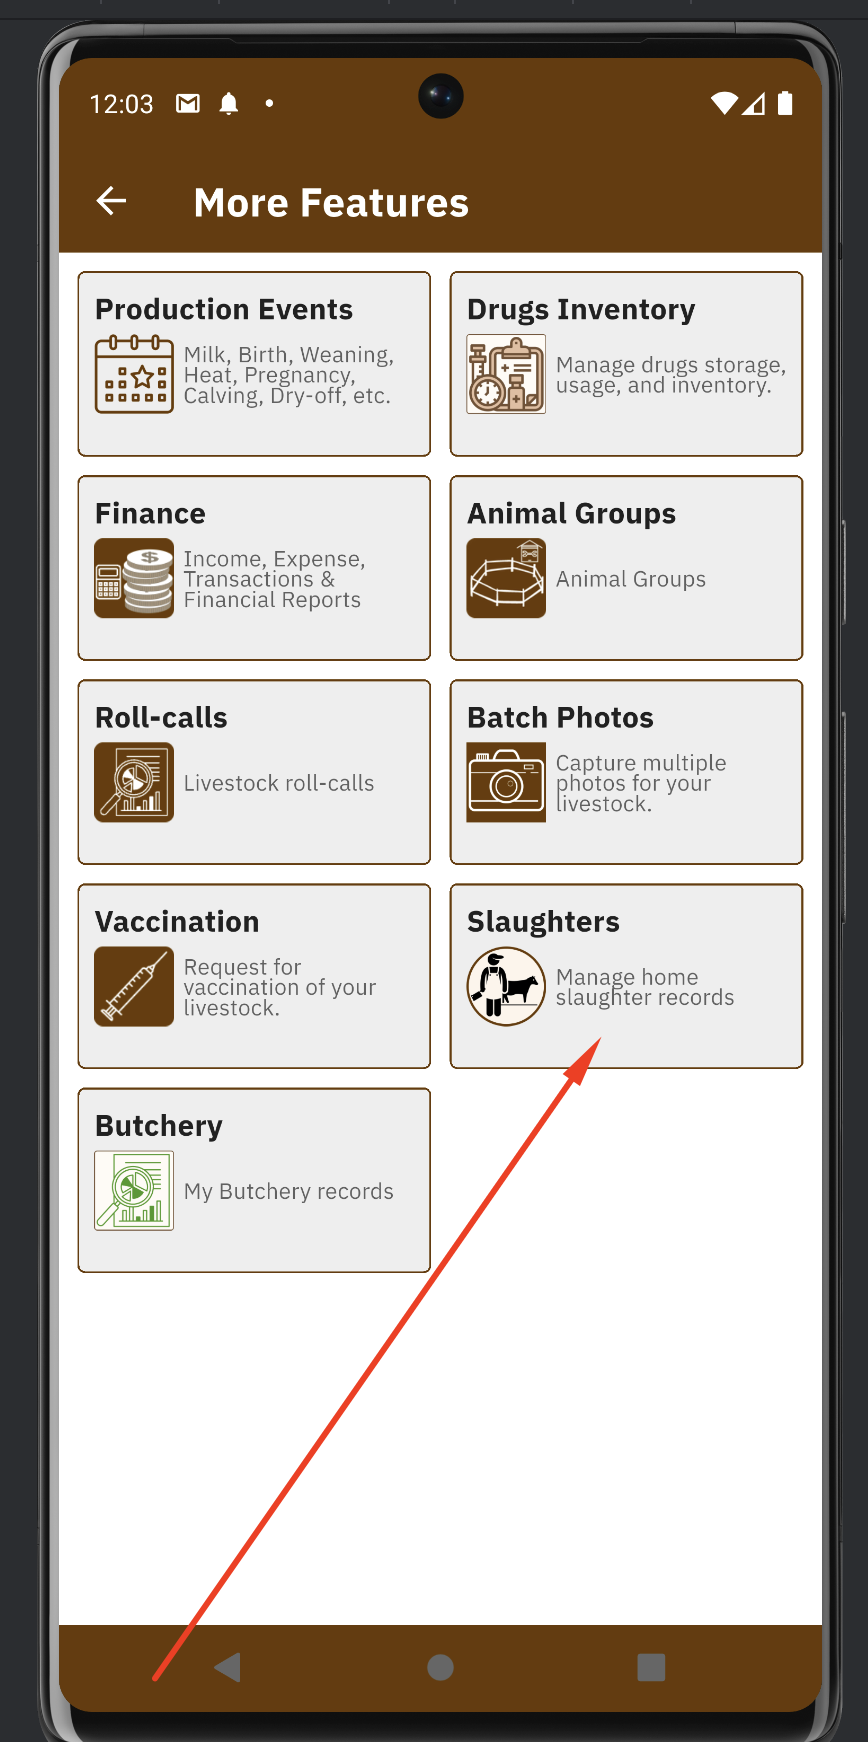
\includegraphics[width=0.45\textwidth]{03_slaughter_records_module.png}
\caption{Slaughter House Officer Accessing Slaughter Records Module}
\label{fig:slaughter_module}
\end{figure}

\begin{figure}[h]
\centering
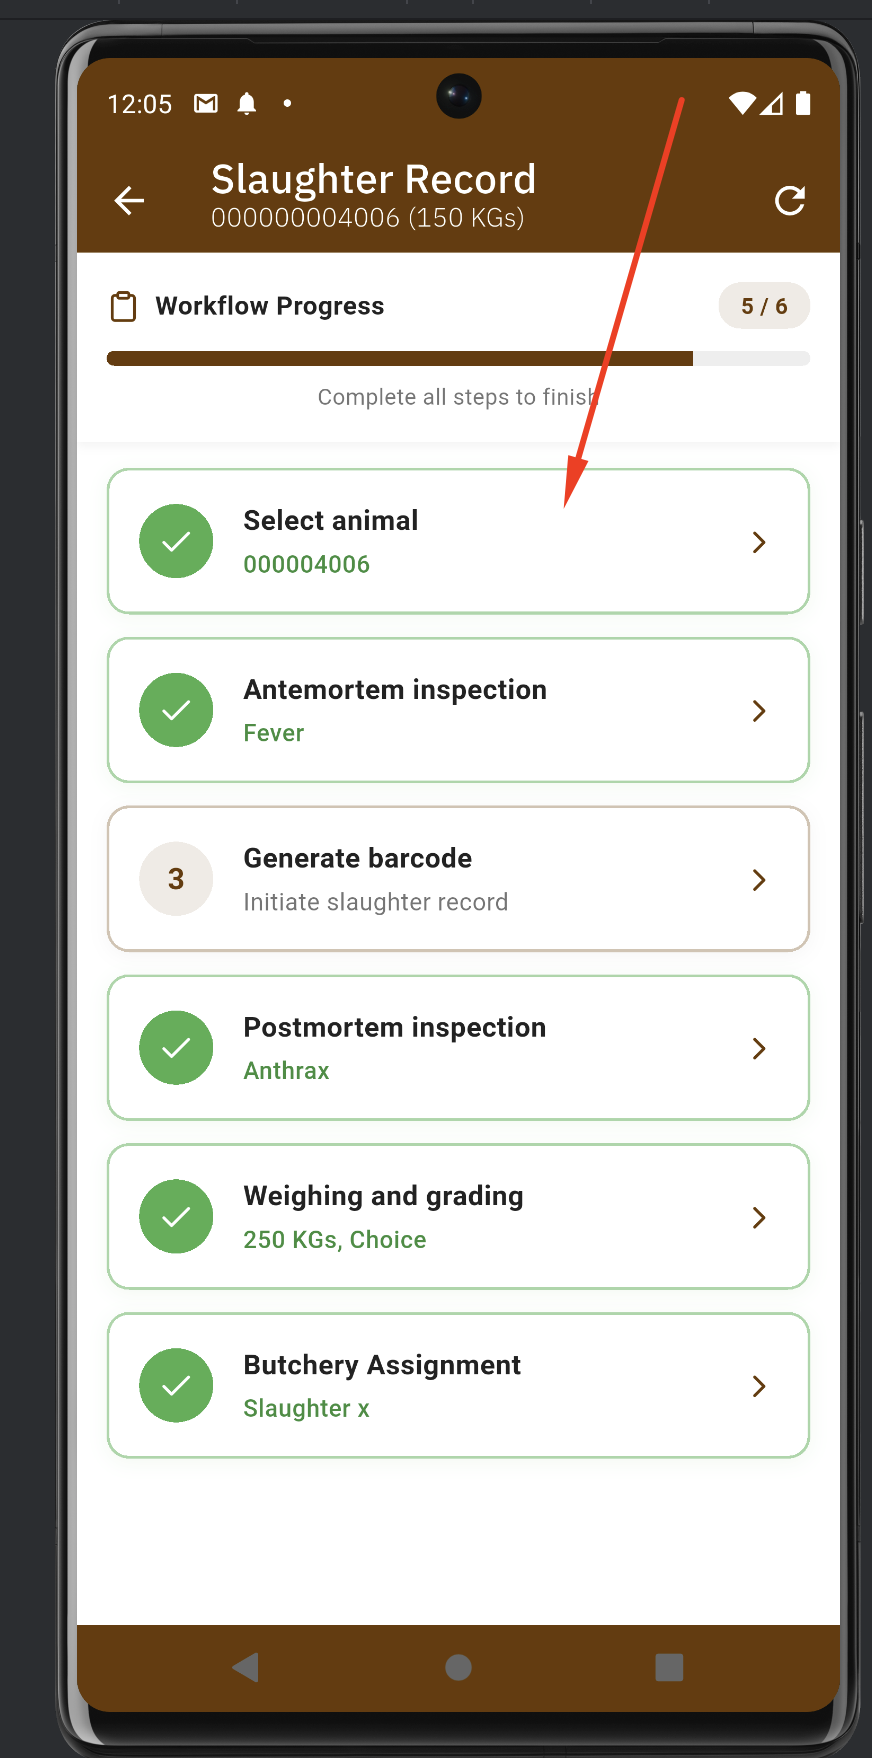
\includegraphics[width=0.45\textwidth]{04_slaughter_record_form.png}
\caption{Creating New Slaughter Record from Movement Permit}
\label{fig:slaughter_form}
\end{figure}

\begin{figure}[h]
\centering
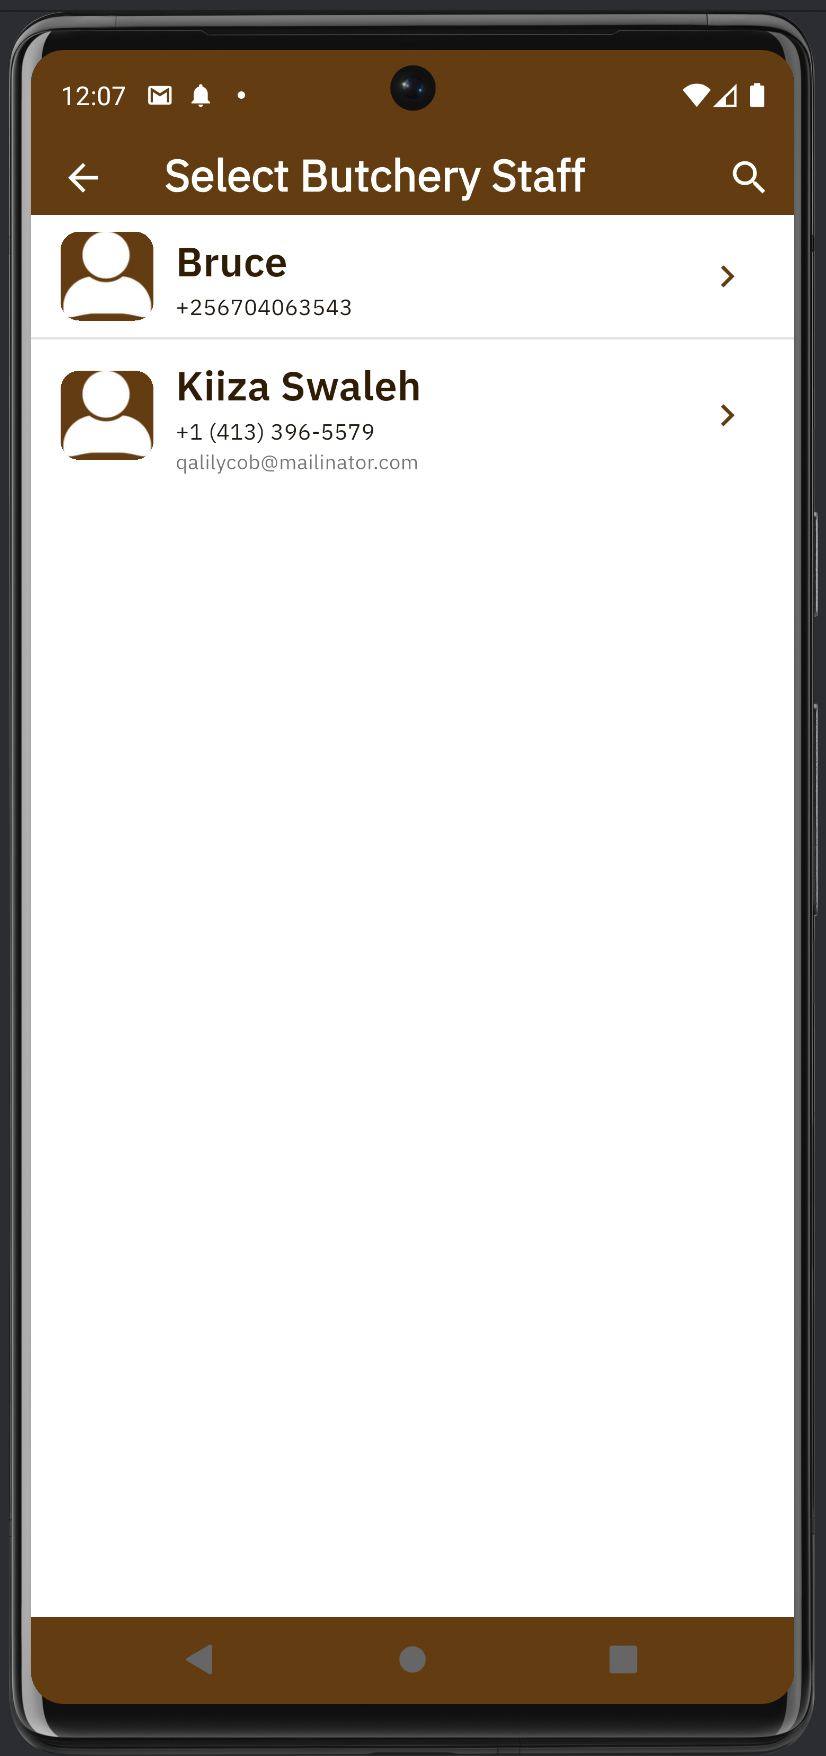
\includegraphics[width=0.45\textwidth]{05_assign_carcass_to_butchery.png}
\caption{Assigning Carcass to Butchery After Slaughter Process}
\label{fig:assign_butchery}
\end{figure}

\section{Butchery Process}

The butchery process transforms whole carcasses into sellable meat products through three distinct stages.

\subsection{Stage 1: Quartering (Primary Breakdown)}

\begin{figure}[h]
\centering
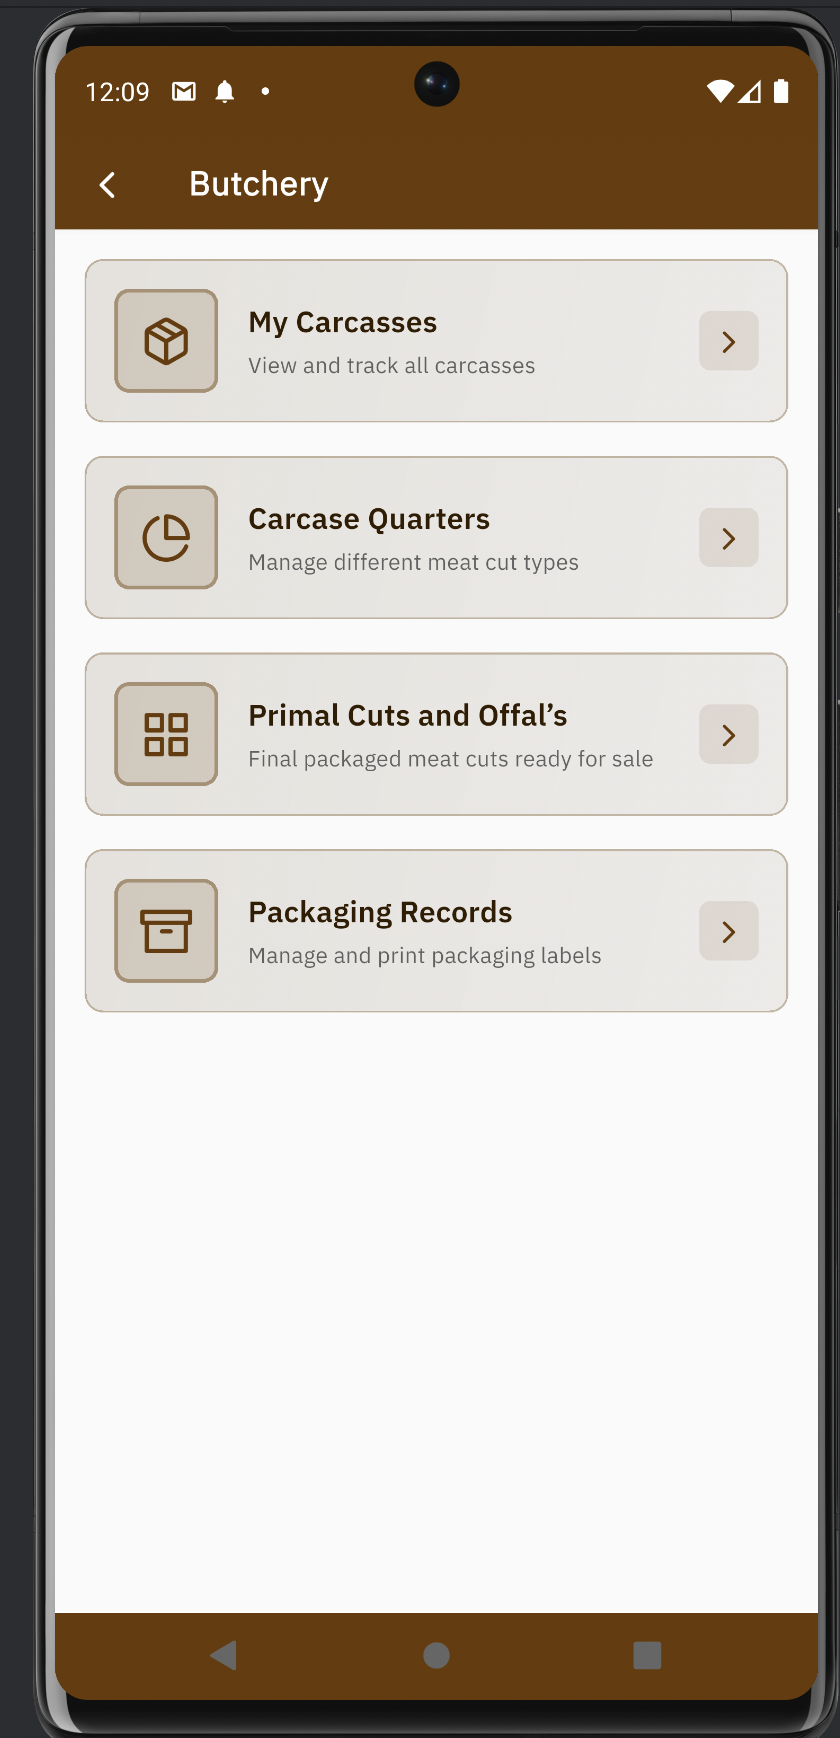
\includegraphics[width=0.45\textwidth]{06_butchery_module_access.png}
\caption{Butchery Officer Accessing Butchery Module}
\label{fig:butchery_access}
\end{figure}

The carcass is divided into four main sections:

\begin{itemize}[leftmargin=*]
    \item \textbf{Fore-Right (FR)} -- Front right portion
    \item \textbf{Fore-Left (FL)} -- Front left portion
    \item \textbf{Hind-Right (HR)} -- Rear right portion
    \item \textbf{Hind-Left (HL)} -- Rear left portion
\end{itemize}

\subsubsection{Quarter Processing}

Each quarter is:

\begin{itemize}[leftmargin=*]
    \item Weighed individually
    \item Recorded as a Slaughter Distribution Record
    \item Tracked for remaining available weight
    \item Assigned for further processing
\end{itemize}

The sum of quarter weights should approximate the original carcass weight (within 5\% tolerance).

\begin{figure}[h]
\centering
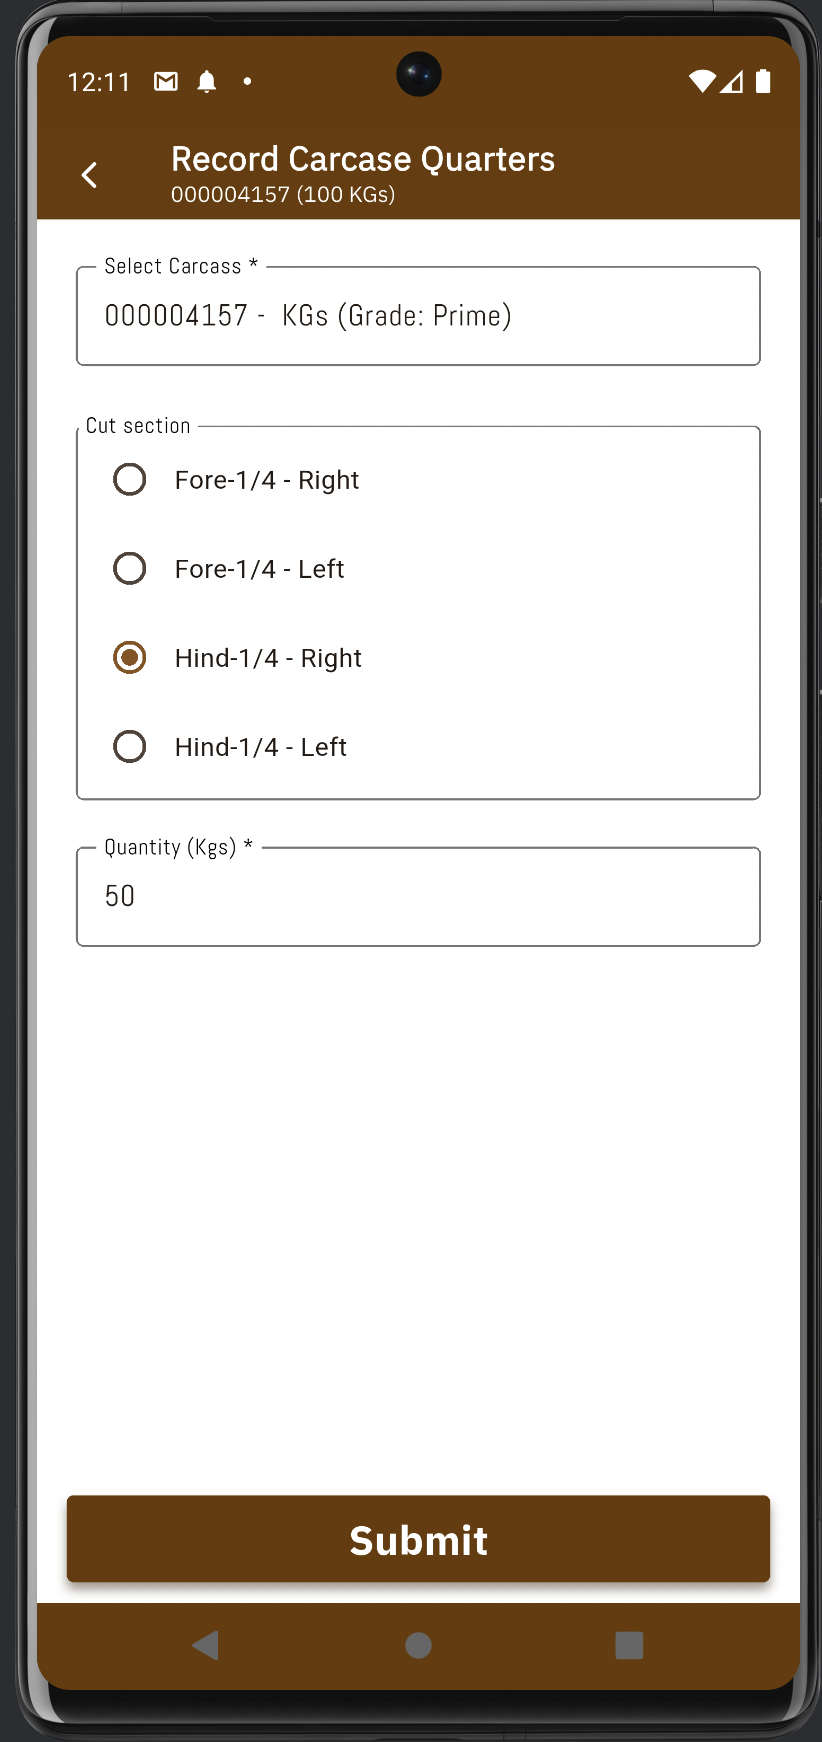
\includegraphics[width=0.45\textwidth]{07_create_quarters.png}
\caption{Creating Quarters from Assigned Carcass}
\label{fig:create_quarters}
\end{figure}

\begin{figure}[h]
\centering
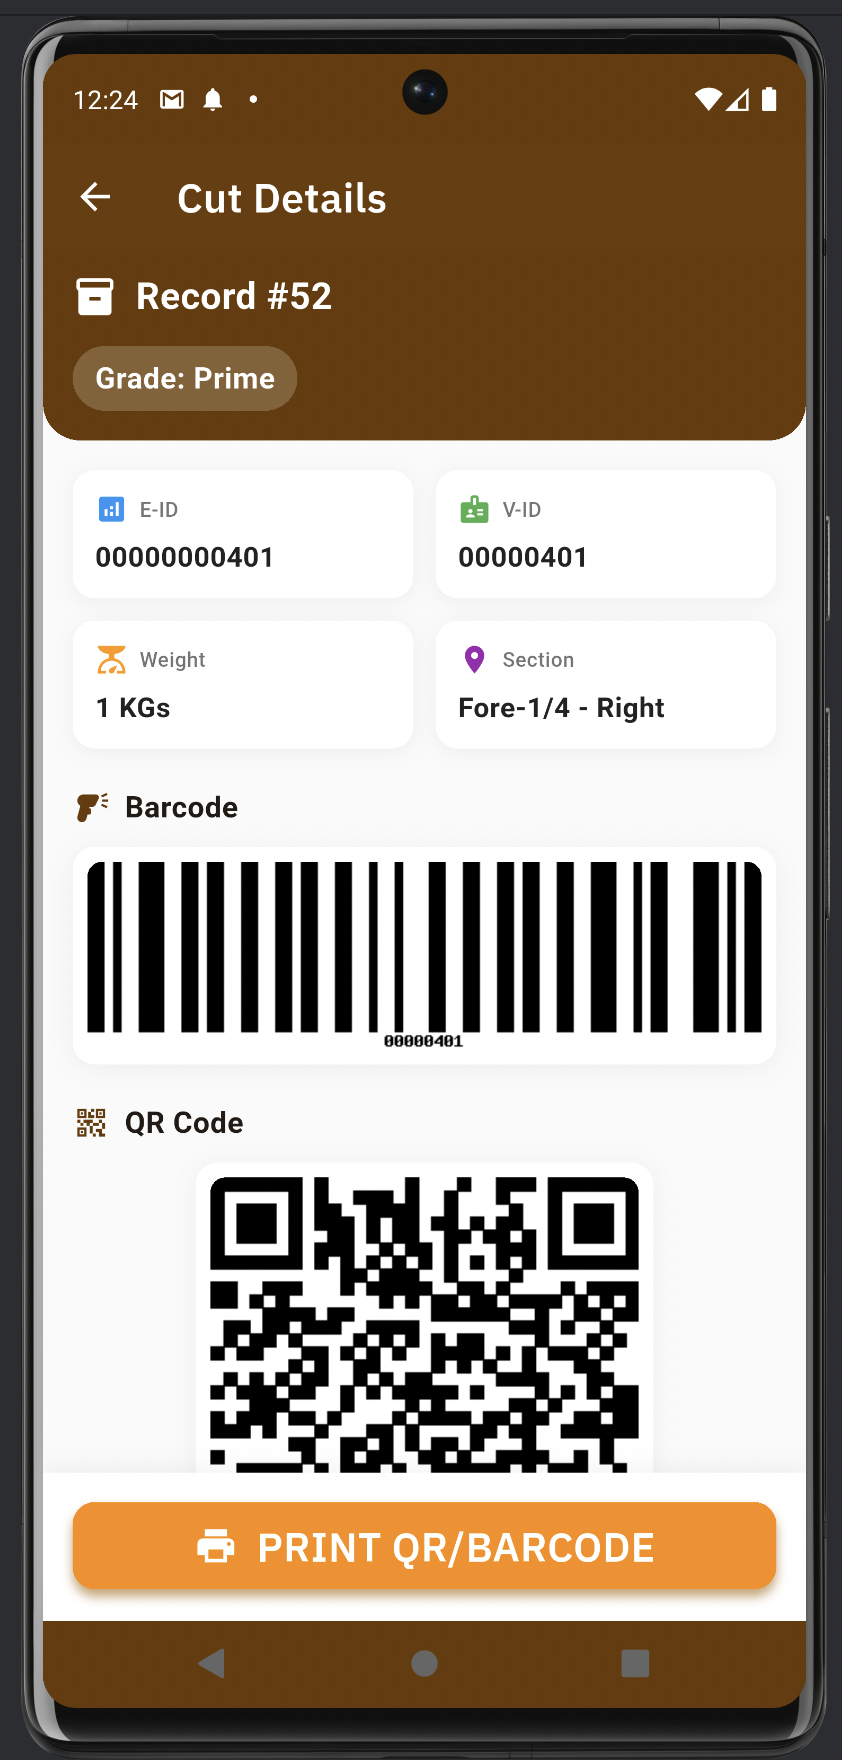
\includegraphics[width=0.45\textwidth]{08_quarter_barcode_label.png}
\caption{Quarter Barcode and QR Code Label for Traceability}
\label{fig:quarter_label}
\end{figure}

\subsection{Stage 2: Cuts (Secondary Breakdown)}

Each quarter is further divided into specific cuts classified as either Primal Cuts or Offal Cuts.

\subsubsection{Primal Cuts (29 types)}

Main meat portions including:

\begin{itemize}[leftmargin=*]
    \item Sirloin/Striploin, T-Bone, Fillet, Rib Eye
    \item Rump, Brisket, Chuck, Topside
    \item Family Steak, Minced Meat, Bones
    \item And 18 additional cut types
\end{itemize}

\subsubsection{Offal Cuts (4 types)}

Organ meats including:

\begin{itemize}[leftmargin=*]
    \item Liver
    \item Heart
    \item Kidneys
    \item Tongue
\end{itemize}

\subsubsection{Cut Recording}

Each cut is recorded with:

\begin{itemize}[leftmargin=*]
    \item Source quarter (FL, FR, HL, HR)
    \item Cut classification (Prime or Offal)
    \item Specific cut name
    \item Weight in kilograms
    \item Barcode for tracking
\end{itemize}

The system automatically reduces the quarter's available weight when cuts are recorded.

\begin{figure}[h]
\centering
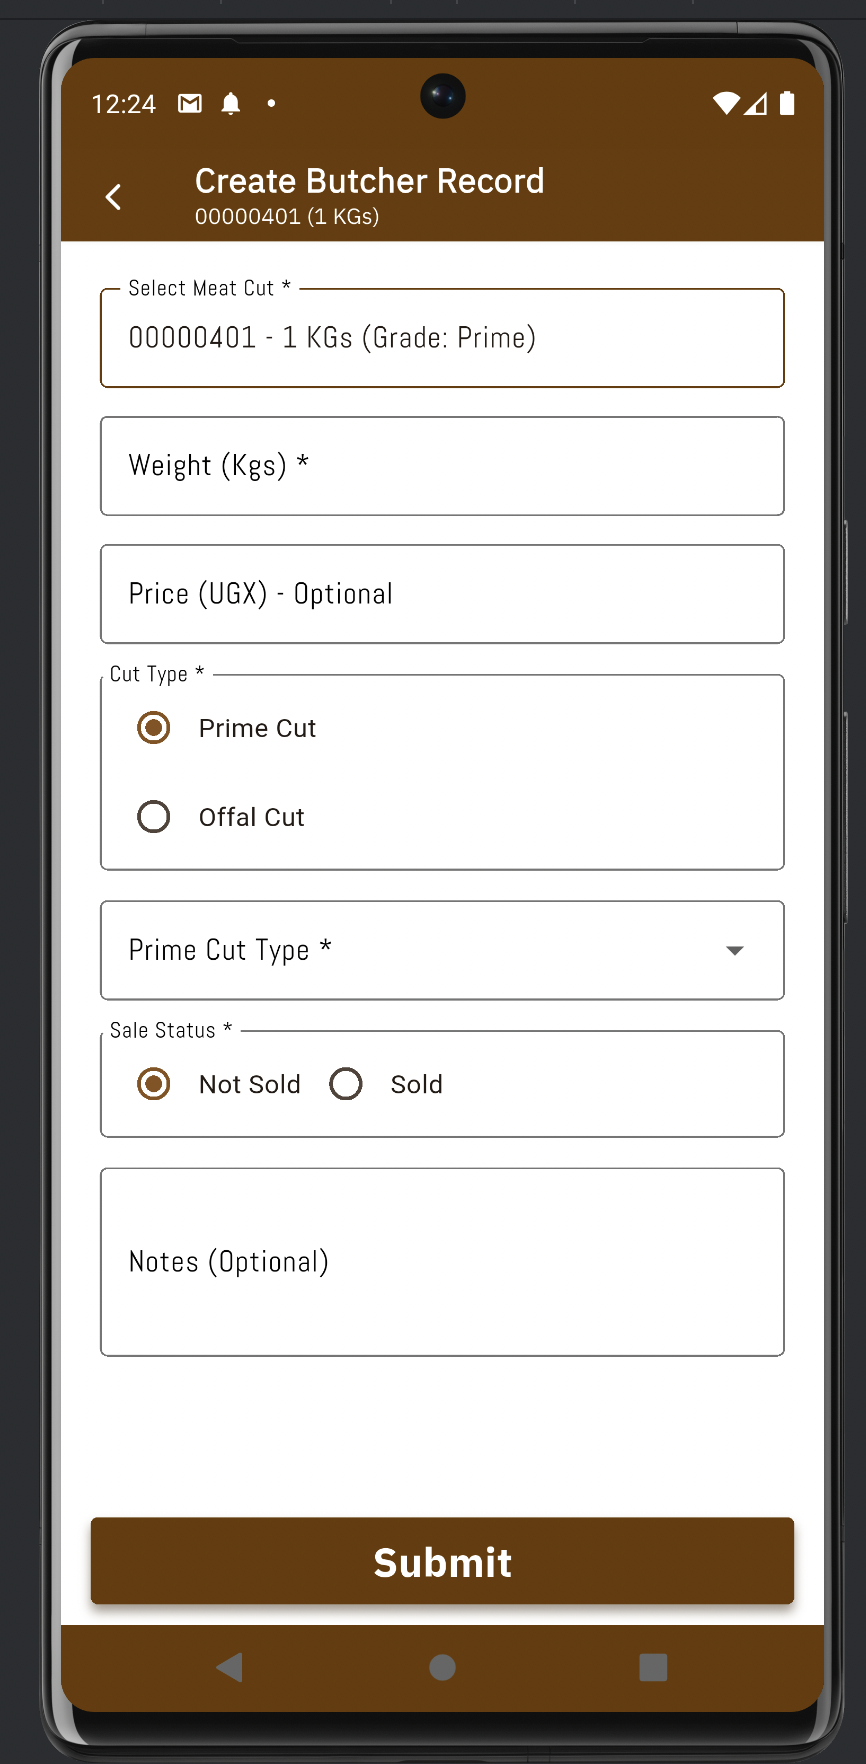
\includegraphics[width=0.45\textwidth]{09_create_cuts_from_quarters.png}
\caption{Creating Prime Cuts and Offal Cuts from Quarters}
\label{fig:create_cuts}
\end{figure}

\subsection{Stage 3: Final Packaging (Butcher Records)}

Cuts are packaged into consumer-ready portions:

\begin{itemize}[leftmargin=*]
    \item Individual package weight recorded
    \item Price assigned
    \item Barcode and QR code generated
    \item Status marked (Available or Sold)
    \item Full traceability maintained
\end{itemize}

\begin{figure}[h]
\centering
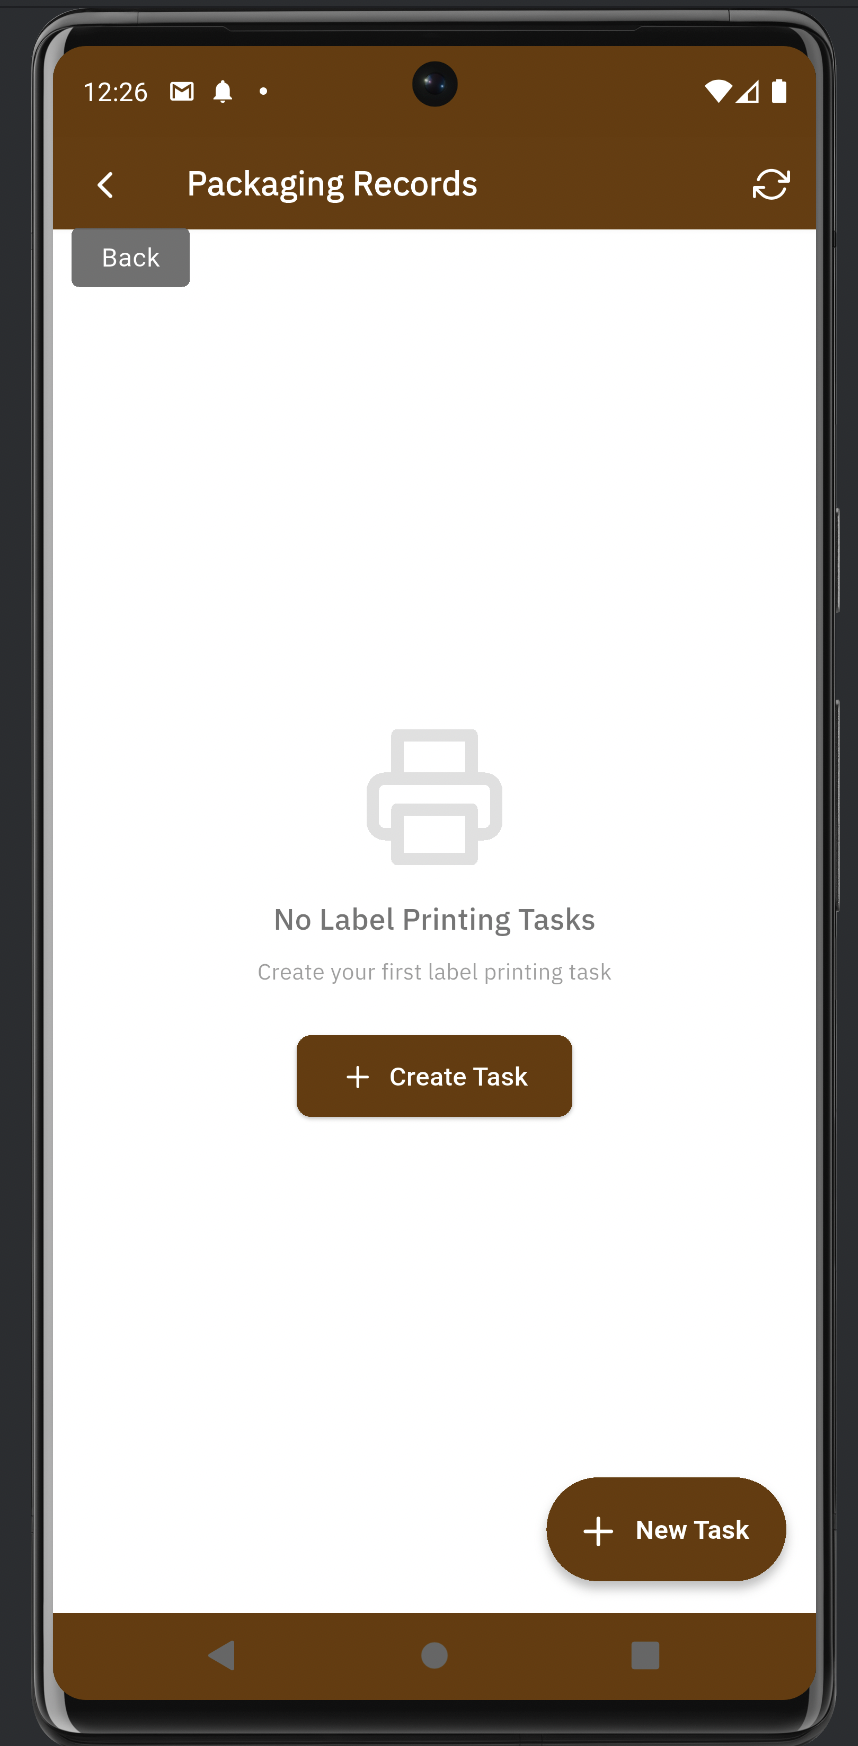
\includegraphics[width=0.45\textwidth]{10_final_packaging_labels.png}
\caption{Creating Final Packaging with Labels and Barcodes}
\label{fig:final_packaging}
\end{figure}

\subsubsection{Sales Recording}

When sold, the system records:

\begin{itemize}[leftmargin=*]
    \item Status updated to ``Sold''
    \item Buyer information recorded
    \item Sale price and date captured
    \item Inventory automatically adjusted
\end{itemize}

\section{Data Relationships}

\subsection{Weight Flow}

The weight tracking flows through the following hierarchy:

\begin{center}
\begin{minipage}{0.8\textwidth}
\begin{verbatim}
Slaughter Record (Carcass)
  |-- Available Weight: Total carcass weight
      |
      v
Slaughter Distribution Records (Quarters)
  |-- 4 quarters created
  |-- Carcass available weight reduced to 0
      |
      v
Slaughter Distribution Records (Cuts)
  |-- Multiple cuts per quarter
  |-- Quarter available weight reduced accordingly
      |
      v
Butcher Records (Final Products)
  |-- Packaged portions from cuts
  |-- Ready for sale with full traceability
\end{verbatim}
\end{minipage}
\end{center}

\subsection{Practical Example}

\subsubsection{Initial Slaughter}
\begin{itemize}[leftmargin=*]
    \item 250 kg carcass recorded
\end{itemize}

\subsubsection{After Quartering}
\begin{itemize}[leftmargin=*]
    \item Fore-Right: 62 kg
    \item Fore-Left: 63 kg
    \item Hind-Right: 65 kg
    \item Hind-Left: 60 kg
    \item Total: 250 kg (matches carcass weight)
\end{itemize}

\subsubsection{Processing Fore-Right Quarter (62 kg)}
\begin{itemize}[leftmargin=*]
    \item Sirloin: 15 kg
    \item T-Bone: 8 kg
    \item Chuck: 20 kg
    \item Bones: 10 kg
    \item Liver: 2 kg
    \item Heart: 2 kg
    \item Waste/Trim: 5 kg
    \item Total: 62 kg (quarter fully processed)
\end{itemize}

\subsubsection{Final Packaging}
\begin{itemize}[leftmargin=*]
    \item 15 packages of Sirloin (1 kg each)
    \item 8 packages of T-Bone (1 kg each)
    \item 20 packages of Chuck (1 kg each)
    \item Each with unique barcode/QR code
\end{itemize}

\section{User Roles}

\subsection{Farmer/Trader}
\begin{itemize}[leftmargin=*]
    \item Applies for movement permits
    \item Selects animals for transport
    \item Tracks permit status
\end{itemize}

\subsection{District Veterinary Officer}
\begin{itemize}[leftmargin=*]
    \item Reviews permit applications
    \item Approves or rejects permits
    \item Monitors district animal movements
\end{itemize}

\subsection{Checkpoint Inspector}
\begin{itemize}[leftmargin=*]
    \item Verifies permits during transit
    \item Inspects animals at checkpoints
    \item Records checkpoint passage
\end{itemize}

\subsection{Slaughter House Officer}
\begin{itemize}[leftmargin=*]
    \item Receives animals with permits
    \item Conducts inspections
    \item Creates slaughter records
    \item Assigns meat grades
\end{itemize}

\subsection{Butcher}
\begin{itemize}[leftmargin=*]
    \item Records quarters and cuts
    \item Manages inventory
    \item Creates final packaged products
    \item Records sales transactions
\end{itemize}

\subsection{System Administrator}
\begin{itemize}[leftmargin=*]
    \item Registers facilities
    \item Manages user accounts
    \item Monitors compliance
    \item Generates reports
\end{itemize}

\section{System Features}

\subsection{Mobile Application}

The mobile application provides:

\begin{itemize}[leftmargin=*]
    \item Movement permit management
    \item Slaughter record creation
    \item Inspection form completion
    \item Barcode generation and scanning
    \item Quarter and cut recording
    \item Sales transaction recording
    \item Full traceability access
\end{itemize}

\subsection{Web Portal}

The web portal offers:

\begin{itemize}[leftmargin=*]
    \item Comprehensive dashboard with statistics
    \item Record management (slaughters, distributions, butcher records)
    \item Advanced filtering and search capabilities
    \item Inventory tracking
    \item Sales reporting
    \item Label generation
    \item Data export capabilities
\end{itemize}

\section{Traceability}

Every meat product maintains complete traceability through the supply chain:

\begin{center}
\begin{minipage}{0.6\textwidth}
\begin{verbatim}
Consumer Product (Butcher Record)
  |
  v
Meat Cut (Slaughter Distribution Record)
  |
  v
Quarter (Slaughter Distribution Record)
  |
  v
Carcass (Slaughter Record)
  |
  v
Live Animal (Movement Permit)
  |
  v
Farm of Origin
\end{verbatim}
\end{minipage}
\end{center}

\subsection{QR Code Information}

Scanning a QR code on any package reveals:

\begin{itemize}[leftmargin=*]
    \item Farm and farmer details
    \item Movement permit information
    \item Slaughter house and date
    \item Veterinary inspection results
    \item Meat grade and weight
    \item Processing history
    \item Complete audit trail
\end{itemize}

\section{Quality Assurance}

Quality control occurs at multiple stages throughout the process:

\begin{enumerate}[leftmargin=*]
    \item \textbf{Farm Level} -- Animal health records and vaccination status
    \item \textbf{Transport} -- Movement permit verification and checkpoint inspections
    \item \textbf{Reception} -- Permit validation and initial assessment
    \item \textbf{Antemortem} -- Live animal veterinary inspection
    \item \textbf{Postmortem} -- Carcass and organ examination
    \item \textbf{Grading} -- Meat quality classification
    \item \textbf{Processing} -- Weight verification and hygiene standards
    \item \textbf{Packaging} -- Proper labeling and traceability codes
    \item \textbf{Sales} -- Transaction recording and buyer documentation
\end{enumerate}

\section{Business Rules}

\subsection{Movement Permits}
\begin{itemize}[leftmargin=*]
    \item Minimum one animal required
    \item All animals must have identification
    \item Destination must be specified
    \item Immutable after approval
    \item Expires after validity period
\end{itemize}

\subsection{Slaughter Records}
\begin{itemize}[leftmargin=*]
    \item Created only from approved permits
    \item Antemortem inspection mandatory
    \item Postmortem required before grading
    \item Cannot complete until all weight distributed
\end{itemize}

\subsection{Quarters}
\begin{itemize}[leftmargin=*]
    \item Must reference valid carcass
    \item Total weights should match carcass ($\pm$5\%)
    \item Four distinct quarters per carcass
    \item Cannot exceed available carcass weight
\end{itemize}

\subsection{Cuts}
\begin{itemize}[leftmargin=*]
    \item Must reference valid quarter
    \item Weight cannot exceed quarter availability
    \item Requires cut type specification
    \item Automatically reduces quarter weight
\end{itemize}

\subsection{Butcher Records}
\begin{itemize}[leftmargin=*]
    \item Created from valid cuts
    \item Cannot exceed source cut weight
    \item Prime or Offal classification required
    \item Sold status is permanent
\end{itemize}

\section{System Benefits}

\subsection{For Farmers}
\begin{itemize}[leftmargin=*]
    \item Official transport documentation
    \item Access to formal markets
    \item Fair pricing based on grades
\end{itemize}

\subsection{For Slaughter Houses}
\begin{itemize}[leftmargin=*]
    \item Digital record keeping
    \item Regulatory compliance
    \item Quality control systems
    \item Efficient operations
\end{itemize}

\subsection{For Butchers}
\begin{itemize}[leftmargin=*]
    \item Inventory management
    \item Sales tracking
    \item Professional labeling
    \item Accurate traceability
\end{itemize}

\subsection{For Consumers}
\begin{itemize}[leftmargin=*]
    \item Origin transparency
    \item Quality verification
    \item Food safety assurance
    \item Veterinary certification access
\end{itemize}

\subsection{For Government}
\begin{itemize}[leftmargin=*]
    \item Disease surveillance
    \item Food safety monitoring
    \item Market regulation
    \item Policy-making data
\end{itemize}

\section{Conclusion}

The Slaughter and Butchery module provides a comprehensive digital solution for meat production management. By connecting all stakeholders in the supply chain and maintaining complete traceability from farm to consumer, the system ensures food safety, regulatory compliance, and market transparency.

This integrated approach strengthens Uganda's livestock sector by providing transparent, accountable, and efficient meat production processes that benefit all participants in the value chain.

\end{document}
